\documentclass[10pt]{beamer}
\usepackage{tcolorbox}
\usepackage{float}
\usepackage{tikz}    
\usepackage{amssymb}
\usetheme[progressbar=frametitle]{metropolis}
\usepackage{appendixnumberbeamer}
\usepackage[normalem]{ulem}
\usepackage{booktabs}
\usepackage[scale=2]{ccicons}
\usepackage[utf8]{inputenc}
\usepackage{soul}
\usepackage{pgfplots}
\usepgfplotslibrary{dateplot}
 \usepackage{relsize}
\usepackage{xspace}
\usepackage{graphicx}
\newcommand{\themename}{\textbf{\textsc{metropolis}}\xspace}

\title{Aprendamos sobre Learnability}
\subtitle{\tiny{Pun intended}}
% \date{\today}
\date{}
\author{Guillermo (Billy) Mosse}
\institute{Exactas, UBA}
% \titlegraphic{\hfill\includegraphics[height=1.5cm]{logo.pdf}}

\newtcolorbox{mybox}[3][]
{
  colframe = #2!25,
  colback  = #2!10,
  coltitle = #2!20!black,  
  title    = #3,
  #1,
}


\begin{document}

\maketitle

%\begin{frame}{Table of contents}
%  \setbeamertemplate{section in toc}[sections numbered]
  %\tableofcontents[hideallsubsections]
%\end{frame}

%\section{Introducción}

%TODO Probably approximately correct learning WIKIPEDIA, machine learning


%TODO PAC LEARNABLE EQUIVALENTE A GLIVENKO CANTELLI https://www.cs.bgu.ac.il/~asml162/wiki.files/ugc-pac.pdf
\begin{frame}[fragile]{¿Qué queremos definir?}

¿Se puede inferir una función de manera computable a partir de finitas entradas?


%\begin{itemize}[<+- | alert@+>]
%    \item This is important
%    \item Now this
%    \item And now this
%  \end{itemize}
\end{frame}


\begin{frame}{¿Qué necesitamos para responder esa pregunta?}
	\begin{itemize}{
	\visible<1->{
		\item ¿De qué bolsa estamos sacando la función? \\
		%De qué bolsa estamos sacando funciones?
	Por ejemplo, si queremos aprender una función $f$ que \textbf{sabemos} que es lineal, se puede aprender con solo 2 datos.}
	}
	\visible<2->{
		\item ¿Cuándo/Cuánto queremos aprender a la función?
		No es lo mismo aprenderla luego de $n$ pasos con $n$ prefijado que en el límite,
		o de manera probabilística.
		}
	
\end{itemize}

	
\end{frame}

\begin{frame}{Learnability in the limit}

\underline{Notación}: Dada $f$ una función, notamos $f^{n}$ a la n-upla de pares $[<x_1,f(x_1)>,\cdots,<x_n,f(x_n)>]$, es decir, a un sample de tamaño n de la función $f$.

\visible<2->{\begin{mybox}{green}{Definición}
Una clase $C$ de funciones total computables se dice que \textbf{se puede aprender en el límite} ("learnable in the limit") $\Leftrightarrow$ existe una función computable total $g : \mathbb{N} \rightarrow \mathbb{N}$ llamada \textbf{aprendedora} ("\st{Alejandro} Learner") tal que $\forall\ f \in C\ \exists\ n_f \in \mathbb{N}$ tal que:

\begin{itemize}

%\item $\mathlarger{\mathlarger{\mathlarger{\mathlarger{\phi_{g(f^{n_f})}}}}}$ \huge{computa a $f$}

\visible<3->{ \Large \item $\phi_{g(f^{n_f})}$ computa a $f$}

\visible<4->{\item $g(f^{n}) = g(f^{n_f})\ \forall n\ \geq n_f$}
\end{itemize}
\end{mybox}}


\visible<5->{
Denotamos $\mathcal{LIM}$ como el conjunto de las clases que se pueden aprender en el límite.}

\visible<6->{\underline{Obs}: podríamos pedir que el sample no venga ordenado.}


\end{frame}


\begin{frame}{¿Qué hay en $\mathcal{LIM}$?}

Trivialmente, $\forall f$ computable, $\{f\} \in \mathcal{LIM}$ vía $g(n) \equiv e$, donde $e$ es el número de programa de $f$.


\visible<2->{Ejercicio: Si $C$ es un conjunto finito de funciones computables, $C \in LIM$}

%\visible<3->{Ejercicio: $\{K\}$, visto como función característica, no está en $LIM$}

\visible<3->{¡Lo interesante es ver clases infinitas de funciones computables!}

\end{frame}


\begin{frame}{Ajustemos la definición}
%https://cs.uwaterloo.ca/~watrous/CS360.Spring2017/Lectures/18.pdf

\begin{mybox}{green}{Definición}
Vamos a decir que una clase de funciones totales $C$ se puede t-aprender en el límite si se puede aprender en el límite vía una función $g$ (total, como antes) tal que $\phi_{g(n)}$ es total $\forall$ n. Llamamos $\mathcal{RTOTAL}$ al conjunto de clases que se pueden t-aprender.
\end{mybox}
%\underline{Obs}: en inglés es "R-learnable in the limit" porque llaman "recursivas" a las computables totales (y "partial recursive" a las parcial computables)

\visible<2->{\underline{Obs}: $\mathcal{RTOTAL}$ $\subset$ $\mathcal{LIM}$ (vía la misma g)}

\end{frame}

%TODO: agregar los recuadros de teoremas.

%TODO contar por que va la R en RTOTAL
\begin{frame}{Caracterización de $\mathcal{RTOTAL}$}

\begin{mybox}{green}{Definición}
$C$ es computablemente enumerable como conjunto de funciones si existe una función "enumeradora" computable $\psi$,
 tal que $\forall\ f\ \in C\ \exists\ i$ tal que $f = \psi_i$
\end{mybox}
\visible<2->{\begin{mybox}{black}{Teorema}
Dada una clase de funciones totales $C$, $C \in \mathcal{RTOTAL} \Leftrightarrow$ $C$ es un subconjunto de \textbf{una familia de funciones totales} computablemente enumerable.
\end{mybox}}

\visible<3->{
	
	dem: ejercicio (?)
	Idea:
	\begin{itemize}
		\item Si $C$ se puede aprender, la función $g$ learner me genera el superset enumerable de $C$.
		\item Si $C$ está generado por $\psi$, la hipótesis que devuelvo para entrada será la primera función que me genera $\psi$ compatible con esa entrada. Eso casi que funciona.
		
%		*En realidad hay que arreglarlo para que $\phi_{g(n)}$ sea siempre total.
		\end{itemize}}
\end{frame}


\begin{frame}{Imagen que le pedí prestada a Gaby Senno}
Para la vuelta:

	\begin{figure}[H]
\centering
\includegraphics[width=0.4\columnwidth]{learning.pdf}
\caption {Luego de ver $f(0)=0, f(1)=0,f(2)=1$, la función learner $g$ devuelve $\psi(i)$,i.e, $\phi_{g(f^3)}(x) = \phi_{\psi(i)}(x)$ \label{figLearn}}
%{Let $\{s_i\}_{i\in\NN}$ be a computable enumeration of a class of (in this case $0,1$-valued) total computable functions. Learning by enumeration works as folllows: after seeing $f(0)=1$, $f(1)=0$ and $f(2)=1$, the guess for (a program comoputing) $f$ will be the first TM in the enumeration whose outputs match those values (in the example, $s_6.$) \label{figLearn}}
\end{figure}

\end{frame}


\begin{frame}{Funciones acotadas temporalmente por una $T$}
\begin{mybox}{green}{Definición}
Dada $T$ una función computable (total), decimos que $f$ es computable en tiempo $O(T(n))$ si para casi todo $n$ $f$ tarda a lo sumo $T(n)$ pasos en computar $T(n)$.
\end{mybox}
\visible<2->{
\begin{mybox}{black}{Proposición}
Dada $T$ como arriba, la clase de funciones $C_T$ computable en tiempo $O(T(n))$ es computablemente enumerable (¡en el sentido de funciones!)
\end{mybox}}

	\visible<3->{
	dem: la idea es dar para cada $i$ una función $f$ que para casi toda entrada $n$ tarde menos de $T(n)$ pasos en computarla.}
	
	\visible<4->{
	Idea:
	
	$\psi(i)(x)$ va a hacer lo siguiente: corre el programa $\phi_i$ con entrada $1$ hasta tiempo $T(1)$. Si no termina, devuelve $0$ (algún número de programa de la función constantemente $0$).}
	
\end{frame}

\begin{frame}{(sigue la demo)}

Si termina, corre $\phi_i$ con entrada $k$ hasta tiempo $T(k)\ \forall\ k \leq x$. Si en algún momento tardo se cumple que $\phi_i(k)$ no terminó a tiempo $T(k)$ devuelve $0$.
	
	Si $\forall\ k\ \phi_i(k)$ tarda el tiempo correcto, devuelve  (el nro de) $\phi_i(x)$.

¿Por qué esto es (casi)* correcto?
	
$\forall\ i$, si $\phi_i \not \in C_T$, entonces $\psi_i$ es 0 ctp (y por lo tanto está en $C_T$). Y si $\phi_i \in C_T$, entonces $\psi_i \equiv \phi_i$.

*Una sutileza que no estoy tratando: por simplicidad, no genero las funciones que en finitas entradas se pasan de tiempo. Eso se arregla cambiando $\psi(i)$ por una $\psi(i,j)$ acorde. $\qed$


\end{frame}

\begin{frame}{Resultado fuerte}

\begin{mybox}{black}{Teorema}
	Teorema: Si $T$ es una función computable, la clase de funciones (totales) computable en tiempo O(T(n)) está en $\mathcal{RTOTAL}$.
\end{mybox}
	\visible<2->{dem: recién probamos que es computablemente enumerable. $\qed$}
\end{frame}


\begin{frame}{Corolarios copados}

Las siguientes clases de funciones están en $\mathcal{RTOTAL}$:

%TODO por que PR mas lentas que ackerman
\begin{itemize}
	\item PR (porque son más lentas que Ackerman)
	\item P, acotando por cualquier exponencial
	\item NP (¡en serio!): $NP \subsetneq EXSPACE = O(2^{p(n)}) space \subsetneq O(2^{e^n}) space \subset O(2^{(2^{e^n})}) time$

% Esto se da porque https://stackoverflow.com/questions/18686121/differences-between-time-complexity-and-space-complexity
% si tengo k lugares, solo puedo tener 2^k configuraciones distintas.
% esto es un chamullo porque necesitas espacio para guardar la cantidad de pasos que hiciste...

	\item BQP*: $BQP \subset EXPTIME = O(2^{p(n)}) \subsetneq O(2^{e^n})$
	\item PSPACE
	\end{itemize}

	
	*donde BQP es la clase de problemas de decisión que se pueden resolver con una computadora cuántica en tiempo polinomial con una probabilidad de error siempre a lo sumo 1/3.

\end{frame}


\begin{frame}{Existen clases que no se pueden aprender}

\begin{mybox}{black}{Teorema}
	Teorema: la clase de funciones computables totales $TOT$ no está en $\mathcal{RTOTAL}$
\end{mybox}
	
	\visible<2->{
	dem: argumento diagonal! Supongamos que $TOT$ está en $\mathcal{RTOTAL}$ vía la función $g : \mathbb{N} \rightarrow \mathbb{N}$.
	
	Defino $f : \mathbb{N} \rightarrow \mathbb{N}$ como:
	$$f(0):=0$$
	$$f(n+1) := \phi_{g(f^n)}(n+1) + 1$$
	
	Claramente $f$ y $\phi_{g(f^n)}$ nunca van a coincidir, para ninguna entrada $f^n$ (basta mirar la entrada $n+1$ para cada n).}
	
% O sea, le paso a g el primer valor de f
% g me devuelve la hipótesis f_0
% defino f(1) = f_0(	1) +1. f \neq f_0
% le paso a g f(0),f(1).
% g me devuelve f_2
% defino f(2) = f_2(2) +1. f \neq f_2
% y así...
	
	\visible<3>{$f$ es total computable, es decir, está en $R$ y $f$ y $\phi_{g(f^n)}$ siempre van a diferir en el valor $n+1$. \qed}


\end{frame}


\begin{frame}{¿Y qué pasa con la unión?}



\begin{tikzpicture}[remember picture,overlay]
   \node[anchor=north east,inner sep=0pt] at (current page.north east)
              {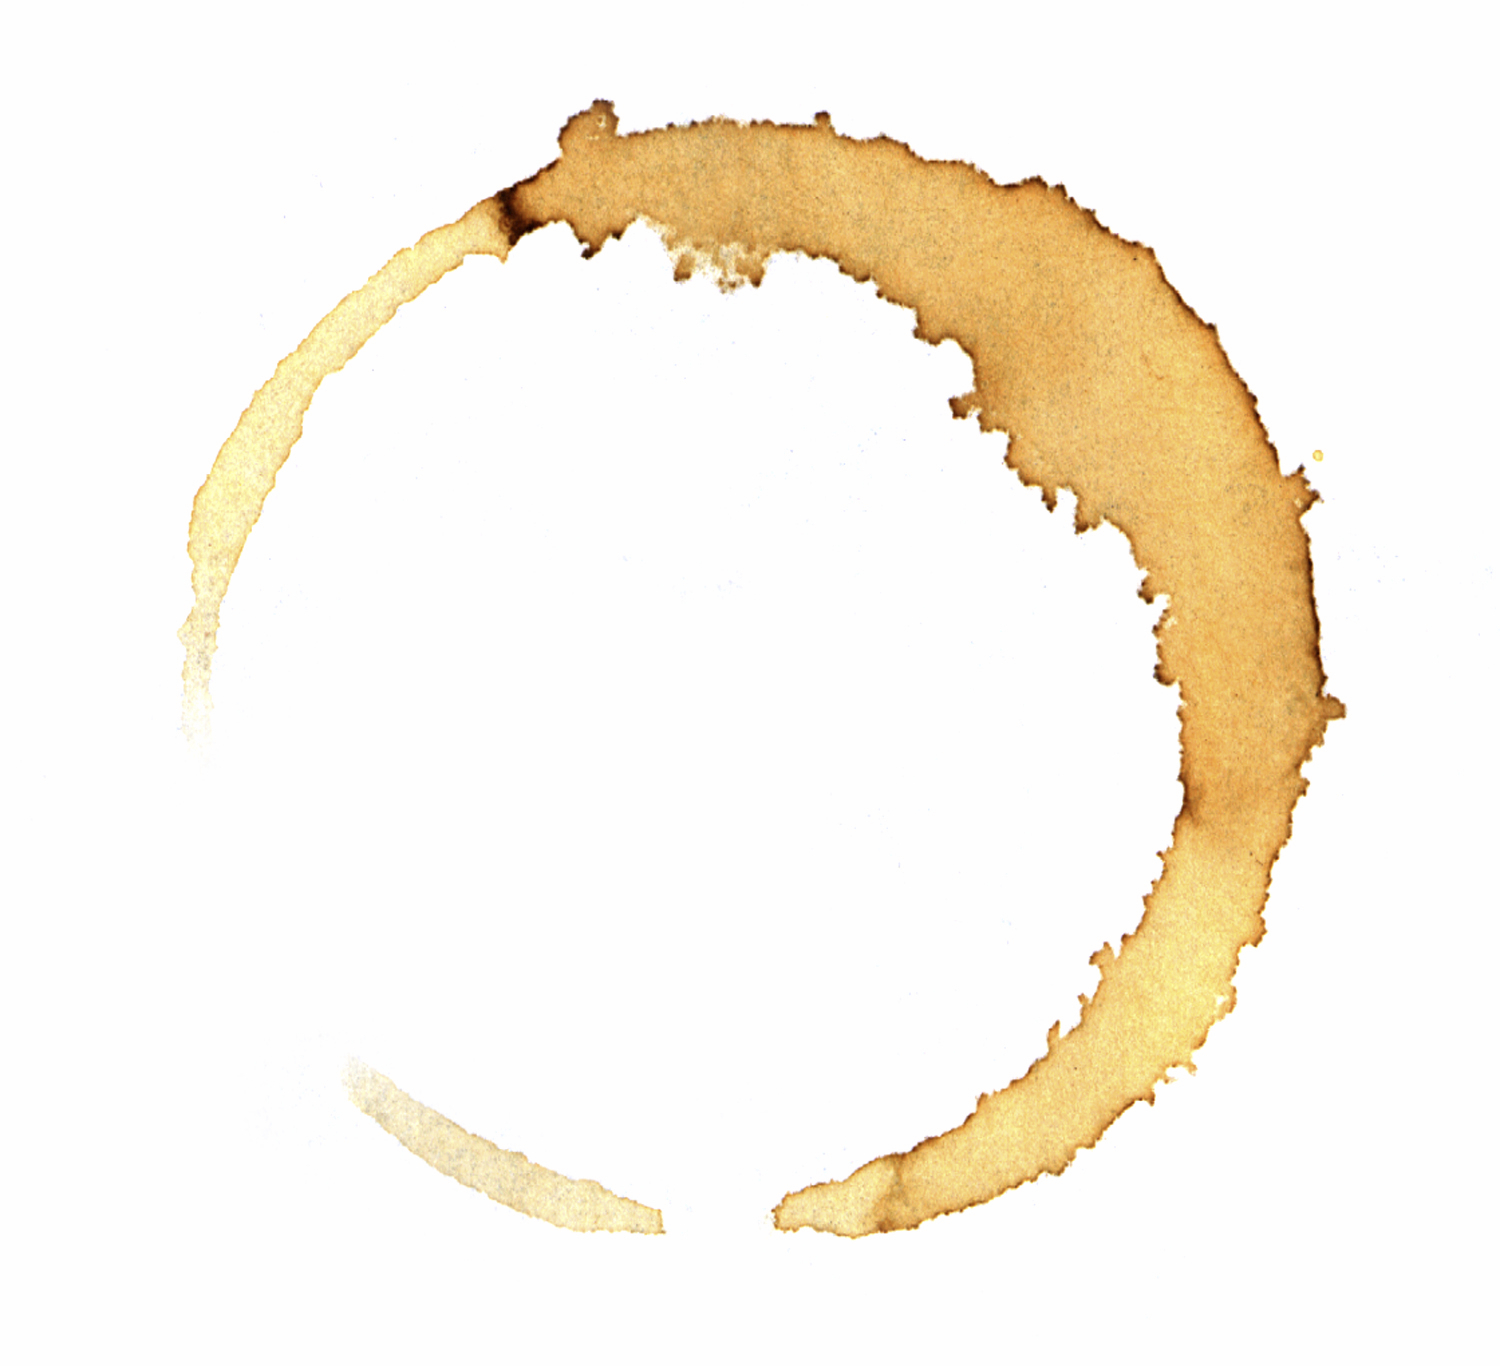
\includegraphics[trim=-15cm 0 4 -2cm, scale=0.7]{coffee.jpg}};
\end{tikzpicture}


\LARGE Si dos clases se pueden aprender, ¿se podrá aprender la unión?


% Y que pasa con LIM? No es cerrado por uniones
% Paper ruso: Two Theorems on the Limiting Synthesis of Functions, Theory of Algorithms and Programs


% http://web.mit.edu/6.863/www/spring2010/readings/gold67limit.pdf

%¿Y si tomo unión numerable? \newline


%TODO esta demo está mal pero quizás se pueda decir algo

%Prop: LIM no es cerrado por unión numerable \newline
%$TOT = \cup A_n$, donde $A_n = \{ f \in TOT : f(x) = 0\ \forall\ x \geq n \}$

%Cada $A_n$ se puede aprender porque luego de n pasos la función se vuelve trivial, pero vimos que TOT no se podía.

%Comentario: LIM tampoco resulta cerrado por uniones.


\end{frame}



%TODO Agregar la siguiente observacion en algun lugar:

% cualquier subconjunto de una clase que se puede aprender, se puede aprender, vía la misma estrategia.





\begin{frame}{Otra manera de aprender}
\begin{mybox}{green}{Definición}
	Una clase $C$ de funciones totales se dice predecible \sout{o aburrida} si existe una función computable total $S$ a la que vamos a llamar "eStrategia" tal que $S(f^n) = f(n+1) \forall f \in C$ y para casi todo $n$ (le permitimos finitos errores).
	
	O sea, pedimos poder predecir casi siempre el siguiente valor de una función.
	
	Denotamos por $NV$ (por "Next Value") 
	\end{mybox}
\end{frame}

\begin{frame}{¡Teorema!}

%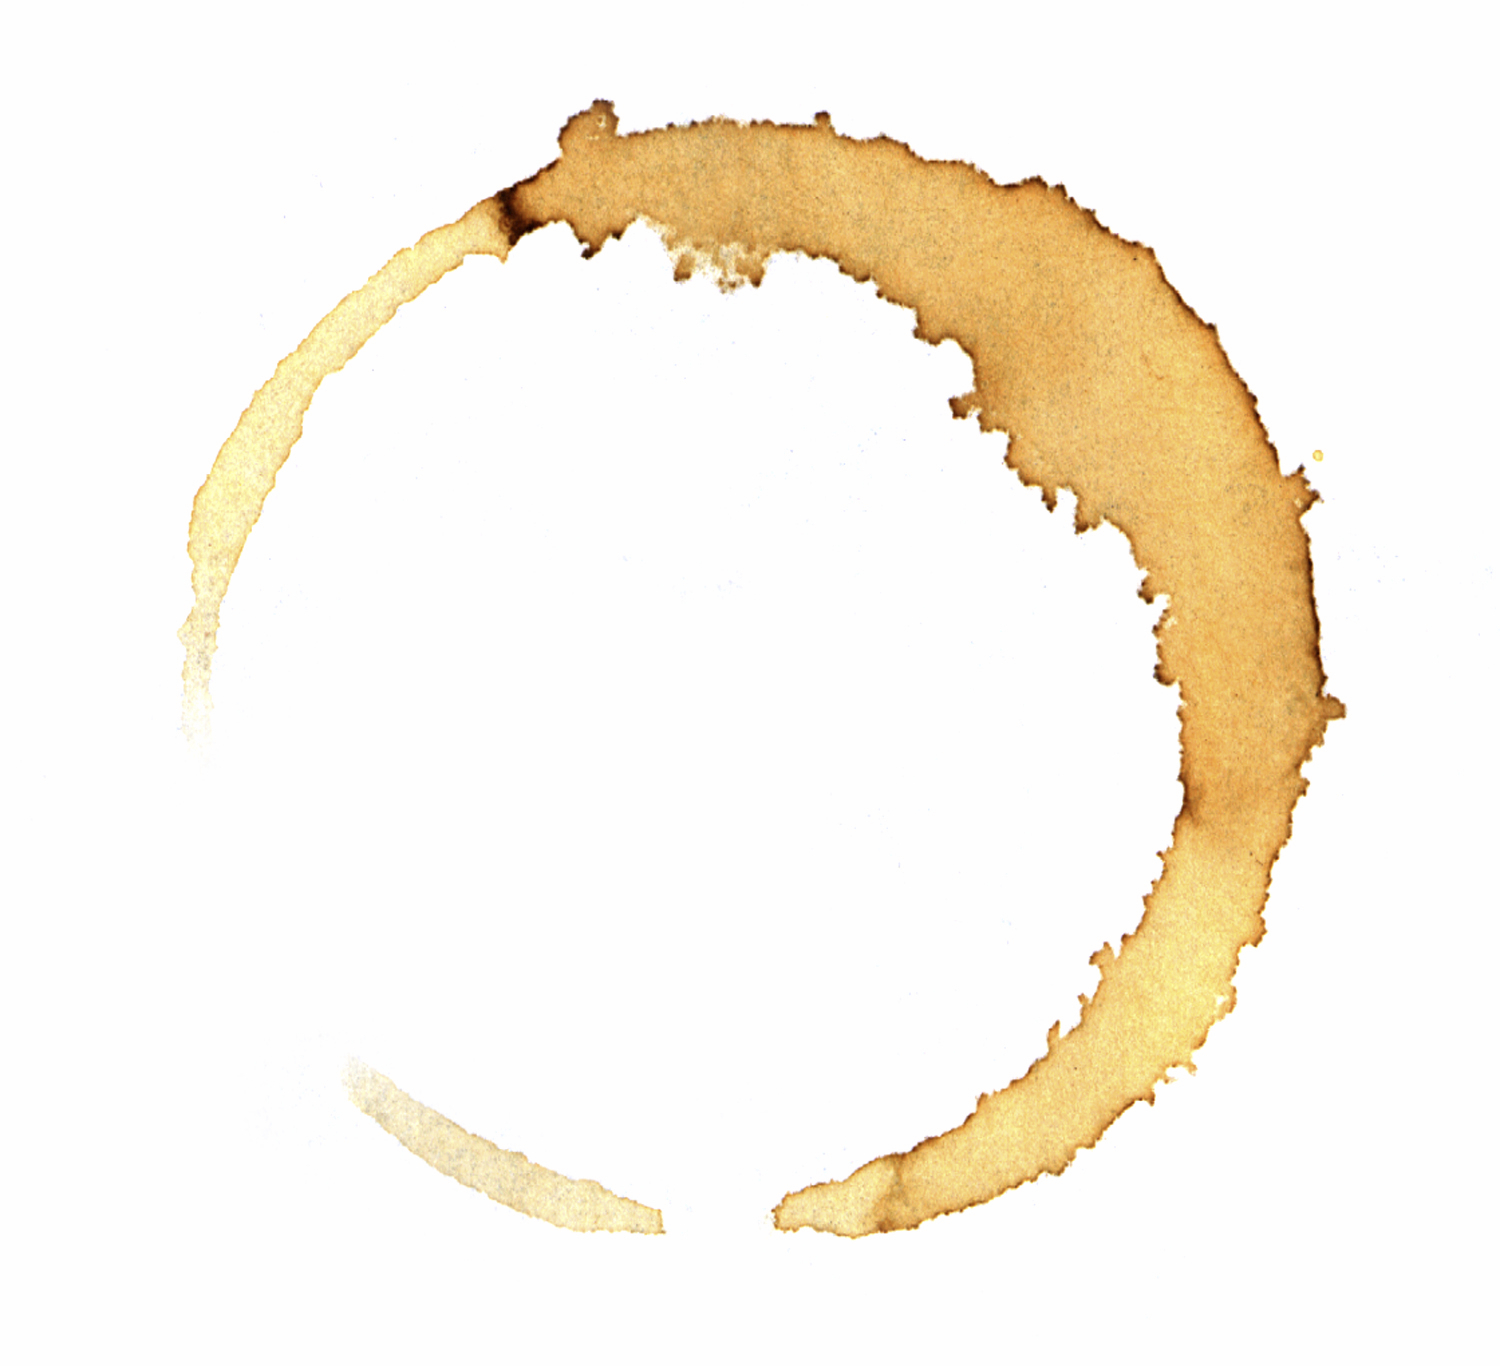
\includegraphics[scale=0.20]{coffee.jpg}


\begin{mybox}{black}{Teorema}
$NV = \mathcal{RTOTAL}$
\end{mybox}

\end{frame}

%TODO no voy a decir nada de esto
%\begin{frame}{¿Es consistencia en las hipótesis mucho pedir?}

% Mirando la demo del teorema que decia que los conjuntos enumerables de funciones se podían aprender, vimos que nunca tirábamos hipótesis que contradecían los datos de entrada

%Definición: una clase $C$ de funciones se dice que se puede aprender de manera consistente si una función $\exists\ g$ learner como antes tal que, además, $\forall\ f \in C, n \in \mathbb{N}$, $\phi_{g(f^n)}(i) = f(i)\ \forall\ i \leq n$ \newline

%Notación que vamos a usar: $\mathcal{LIM_{CONS}}$, $\mathcal{TOTAL_{CONS}}$


%¿Cambiará algo? ¡Veamos a dónde nos lleva esto!

%\end{frame}



%TODO R-TOTAL SE DEFINIA CON EL NUMERO DE FUNCION? RESPUESTA: SI. arreglar
\begin{frame}{Otra manera más de aprender}
	\begin{mybox}{green}{Definición}
	Convergencia semántica en el límite con anomalías: decimos que una clase $C$ se puede aprender correctamente en el límite, pero con $a$ anomalías si $\exists g / \forall\ f\ \in\ C$,
	\begin{itemize}
		\item $\forall\ n\ \in\ \mathbb{N} g(n)$ está definida (esto no cambia)
		\item $\exists\ j \in \mathbb{N}$ tal que $\phi_{S(f^n)} = f\ \forall n \geq n_0$.
	\end{itemize}
	\end{mybox}
	
	\visible<2->{Notación: $C \in \mathcal{BC}$}
	
	\visible<3->{Comentario: TOT$\not \in \mathcal{BC}$. Además no es cerrado por uniones finitas.}

\end{frame}

%TODO R-TOTAL SE DEFINIA CON EL NUMERO DE FUNCION? RESPUESTA: SI. arreglar
\begin{frame}{Última}
	Notación: Dado $a \in \mathbb{N}, f =^a g$ sii $f(x) = g(x)\ \forall\ x \geq a$. Para a = *, pedimos igualdad para todo x salvo finitos.
	
	
	\visible<2->{\begin{mybox}{green}{Definición}
	Convergencia en el límite con anomalías: decimos que una clase $C$ se puede aprender correctamente en el límite, pero con $a$ anomalías si $\exists\ g /\ \forall\ f\ \in\ C$,
	\begin{itemize}
		\item $\forall\ n\ \in\ \mathbb{N} g(n)$ está definida (esto no cambia)
		\item $\exists j \in \mathbb{N} / \phi_j =^a f$ y $S(f^n)$ converge a j.
	\end{itemize}
	\end{mybox}}
	
	\visible<3>{
	
	Más notación: $C \in \mathcal{LIM}^a$.}
	
	
	\visible<4->{Observación: $\mathcal{LIM}^0=\mathcal{LIM}$}

\end{frame}

\begin{frame}{Me encanta decir cosas sin demostrarlas}


\begin{mybox}{black}{Teorema}
$$\mathcal{LIM} \subsetneq \mathcal{LIM}^1 \subsetneq \mathcal{LIM}^2 \subsetneq \mathcal{LIM}^3 \subsetneq ... \bigcup\limits_{a \in \mathbb{N}} \mathcal{LIM}^a \subsetneq \mathcal{LIM}^* \subsetneq BC$$
\end{mybox}

\visible<2->{\begin{mybox}{black}{Teorema}
$$\mathcal{BC} \subsetneq \mathcal{BC}^1 \subsetneq \mathcal{BC}^2 \subsetneq \mathcal{BC}^3 \subsetneq ... \bigcup\limits_{a \in \mathbb{N}} \mathcal{BC}^a \subsetneq \mathcal{BC}^*$$
\end{mybox}}

\visible<3->{\begin{mybox}{black}{Teorema}
$TOT \in BC^*$
\end{mybox}}


\end{frame}


\begin{frame}{Fin}

Preguntas? \bigskip \bigskip


\includegraphics[scale=0.2]{alan.jpg}
\indent\ If Alan was alive, he'd be so happy about gay marriage that he would buy \color{orange}Tu\color{blue}rings\color{black}!
\includegraphics[scale=0.015]{tu.png}

Right? Right?! ... I'll see myself out.

\end{frame}
















\iffalse

\begin{frame}[fragile]{Sections}
  Sections group slides of the same topic

  \begin{verbatim}    \section{Elements}\end{verbatim}

  for which \themename provides a nice progress indicator \ldots
\end{frame}

\section{Titleformats}

\begin{frame}{Metropolis titleformats}
	\themename supports 4 different titleformats:
	\begin{itemize}
		\item Regular
		\item \textsc{Smallcaps}
		\item \textsc{allsmallcaps}
		\item ALLCAPS
	\end{itemize}
	They can either be set at once for every title type or individually.
\end{frame}

{
    \metroset{titleformat frame=smallcaps}
\begin{frame}{Small caps}
	This frame uses the \texttt{smallcaps} titleformat.

	\begin{alertblock}{Potential Problems}
		Be aware, that not every font supports small caps. If for example you typeset your presentation with pdfTeX and the Computer Modern Sans Serif font, every text in smallcaps will be typeset with the Computer Modern Serif font instead.
	\end{alertblock}
\end{frame}
}

{
\metroset{titleformat frame=allsmallcaps}
\begin{frame}{All small caps}
	This frame uses the \texttt{allsmallcaps} titleformat.

	\begin{alertblock}{Potential problems}
		As this titleformat also uses smallcaps you face the same problems as with the \texttt{smallcaps} titleformat. Additionally this format can cause some other problems. Please refer to the documentation if you consider using it.

		As a rule of thumb: Just use it for plaintext-only titles.
	\end{alertblock}
\end{frame}
}

{
\metroset{titleformat frame=allcaps}
\begin{frame}{All caps}
	This frame uses the \texttt{allcaps} titleformat.

	\begin{alertblock}{Potential Problems}
		This titleformat is not as problematic as the \texttt{allsmallcaps} format, but basically suffers from the same deficiencies. So please have a look at the documentation if you want to use it.
	\end{alertblock}
\end{frame}
}

\section{Elements}

\begin{frame}

Desde la pagina 15 hay distintas definiciones de learnability con resultados

Algun ejemplo: K se puede aprender, cualquier computable se puede aprender....
que significa aprender clases de funciones

R-Total teorema 2.5.5 gaby equivalencia 

\end{frame}




%TODO hacer diagrama con LIM, TOTAL, RTOTAL, y uno mas diciendo quien es mas fuerte y que se gana y que se pierde.
%TODO no, mejor hacer círculos




















\begin{frame}[fragile]{Typography}
      \begin{verbatim}The theme provides sensible defaults to
\emph{emphasize} text, \alert{accent} parts
or show \textbf{bold} results.\end{verbatim}

  \begin{center}becomes\end{center}

  The theme provides sensible defaults to \emph{emphasize} text,
  \alert{accent} parts or show \textbf{bold} results.
\end{frame}

\begin{frame}{Font feature test}
  \begin{itemize}
    \item Regular
    \item \textit{Italic}
    \item \textsc{SmallCaps}
    \item \textbf{Bold}
    \item \textbf{\textit{Bold Italic}}
    \item \textbf{\textsc{Bold SmallCaps}}
    \item \texttt{Monospace}
    \item \texttt{\textit{Monospace Italic}}
    \item \texttt{\textbf{Monospace Bold}}
    \item \texttt{\textbf{\textit{Monospace Bold Italic}}}
  \end{itemize}
\end{frame}


\begin{frame}{Lists}
  \begin{columns}[T,onlytextwidth]
    \column{0.33\textwidth}
      Items
      \begin{itemize}
        \item Milk \item Eggs \item Potatos
      \end{itemize}

    \column{0.33\textwidth}
      Enumerations
      \begin{enumerate}
        \item First, \item Second and \item Last.
      \end{enumerate}

    \column{0.33\textwidth}
      Descriptions
      \begin{description}
        \item[PowerPoint] Meeh. \item[Beamer] Yeeeha.
      \end{description}
  \end{columns}
\end{frame}
\begin{frame}{Animation}
  \begin{itemize}[<+- | alert@+>]
    \item \alert<4>{This is\only<4>{ really} important}
    \item Now this
    \item And now this
  \end{itemize}
\end{frame}

\begin{frame}{Figures}
  \begin{figure}
    \newcounter{density}
    \setcounter{density}{20}
    \begin{tikzpicture}
      \def\couleur{alerted text.fg}
      \path[coordinate] (0,0)  coordinate(A)
                  ++( 90:5cm) coordinate(B)
                  ++(0:5cm) coordinate(C)
                  ++(-90:5cm) coordinate(D);
      \draw[fill=\couleur!\thedensity] (A) -- (B) -- (C) --(D) -- cycle;
      \foreach \x in {1,...,40}{%
          \pgfmathsetcounter{density}{\thedensity+20}
          \setcounter{density}{\thedensity}
          \path[coordinate] coordinate(X) at (A){};
          \path[coordinate] (A) -- (B) coordinate[pos=.10](A)
                              -- (C) coordinate[pos=.10](B)
                              -- (D) coordinate[pos=.10](C)
                              -- (X) coordinate[pos=.10](D);
          \draw[fill=\couleur!\thedensity] (A)--(B)--(C)-- (D) -- cycle;
      }
    \end{tikzpicture}
    \caption{Rotated square from
    \href{http://www.texample.net/tikz/examples/rotated-polygons/}{texample.net}.}
  \end{figure}
\end{frame}

\begin{frame}{Tables}
  \begin{table}
    \caption{Largest cities in the world (source: Wikipedia)}
    \begin{tabular}{lr}
      \toprule
      City & Population\\
      \midrule
      Mexico City & 20,116,842\\
      Shanghai & 19,210,000\\
      Peking & 15,796,450\\
      Istanbul & 14,160,467\\
      \bottomrule
    \end{tabular}
  \end{table}
\end{frame}
\begin{frame}{Blocks}
  Three different block environments are pre-defined and may be styled with an
  optional background color.

  \begin{columns}[T,onlytextwidth]
    \column{0.5\textwidth}
      \begin{block}{Default}
        Block content.
      \end{block}

      \begin{alertblock}{Alert}
        Block content.
      \end{alertblock}

      \begin{exampleblock}{Example}
        Block content.
      \end{exampleblock}

    \column{0.5\textwidth}

      \metroset{block=fill}

      \begin{block}{Default}
        Block content.
      \end{block}

      \begin{alertblock}{Alert}
        Block content.
      \end{alertblock}

      \begin{exampleblock}{Example}
        Block content.
      \end{exampleblock}

  \end{columns}
\end{frame}

%\begin{frame}{Math}
%  \begin{equation*}
%    e = \lim_{n\to \infty} \left(1 + \frac{1}{n}\right)^n
%  \end{equation*}
%\end{frame}
\begin{frame}{Line plots}
  \begin{figure}
    \begin{tikzpicture}
      \begin{axis}[
        mlineplot,
        width=0.9\textwidth,
        height=6cm,
      ]

        \addplot {sin(deg(x))};
        \addplot+[samples=100] {sin(deg(2*x))};

      \end{axis}
    \end{tikzpicture}
  \end{figure}
\end{frame}

\begin{frame}{Bar charts}
  \begin{figure}
    \begin{tikzpicture}
      \begin{axis}[
        mbarplot,
        xlabel={Foo},
        ylabel={Bar},
        width=0.9\textwidth,
        height=6cm,
      ]

      \addplot plot coordinates {(1, 20) (2, 25) (3, 22.4) (4, 12.4)};
      \addplot plot coordinates {(1, 18) (2, 24) (3, 23.5) (4, 13.2)};
      \addplot plot coordinates {(1, 10) (2, 19) (3, 25) (4, 15.2)};

      \legend{lorem, ipsum, dolor}

      \end{axis}
    \end{tikzpicture}
  \end{figure}
\end{frame}

\begin{frame}{Quotes}
  \begin{quote}
    Veni, Vidi, Vici
  \end{quote}
\end{frame}

{%
\setbeamertemplate{frame footer}{My custom footer}
\begin{frame}[fragile]{Frame footer}
    \themename defines a custom beamer template to add a text to the footer. It can be set via
    \begin{verbatim}\setbeamertemplate{frame footer}{My custom footer}\end{verbatim}
\end{frame}
}

%\begin{frame}{References}
%  Some references to showcase [allowframebreaks] \cite{knuth92,ConcreteMath,Simpson,Er01,greenwade93}
%\end{frame}

%\section{Conclusion}

\begin{frame}{Summary}

  Get the source of this theme and the demo presentation from

  \begin{center}\url{github.com/matze/mtheme}\end{center}

  The theme \emph{itself} is licensed under a
  \href{http://creativecommons.org/licenses/by-sa/4.0/}{Creative Commons
  Attribution-ShareAlike 4.0 International License}.

  %\begin{center}\ccbysa\end{center}

\end{frame}

\begin{frame}[standout]
  Questions?
\end{frame}

\appendix

\begin{frame}[fragile]{Backup slides}
  Sometimes, it is useful to add slides at the end of your presentation to
  refer to during audience questions.

  The best way to do this is to include the \verb|appendixnumberbeamer|
  package in your preamble and call \verb|\appendix| before your backup slides.

  \themename will automatically turn off slide numbering and progress bars for
  slides in the appendix.
\end{frame}
\fi

%\begin{frame}[allowframebreaks]{References}
%  \bibliography{demo}
%  \bibliographystyle{abbrv}

%\end{frame}

\end{document}
